% Wits BSc Honours research report: supervisor feedback draft, 22 Oct 2026.
% LaTeX source remains editable. Counts are preliminary unless explicitly marked row-checked.
\documentclass[journal,10pt,twoside]{IEEEtran}
\usepackage[T1]{fontenc}
\usepackage[utf8]{inputenc}
\usepackage{newtxtext,newtxmath}
\usepackage{graphicx}
\usepackage{amsmath}
\usepackage{booktabs,tabularx,array}
\usepackage{microtype}
\usepackage{url}
\usepackage{balance}
\usepackage{tikz}
\usepackage{enumitem}
\usepackage{hyperref}
\usepackage{natbib}
\usetikzlibrary{positioning,arrows.meta}
\hypersetup{colorlinks=true,linkcolor=blue!55!black,urlcolor=blue!55!black,citecolor=blue!55!black}
\setlist[itemize]{leftmargin=*,nosep,topsep=1pt}
\bibliographystyle{apalike}
\renewcommand{\bibname}{References}
\newcommand{\drafttag}{\emph{Preliminary; not independently re-scanned or fully human-adjudicated.}}
\newcommand{\ncase}[1]{\texttt{#1}}
\setlength{\textfloatsep}{9pt plus 2pt minus 2pt}
\setlength{\floatsep}{7pt plus 2pt minus 1pt}
\setlength{\intextsep}{7pt plus 2pt minus 1pt}
\begin{document}
\title{\vspace{2pt}\includegraphics[width=0.115\textwidth]{images/witslogonew.png}\\[4pt]
\Large\bfseries From GitHub Issues to Security-Relevant Implementation Choices:\\An Exploratory Study of Agent-Associated Pull Requests}
\author{Arno Strauss, Student No.~2613224\\[-2pt]
\small School of Computer Science and Applied Mathematics, University of the Witwatersrand\\[-2pt]
\small Co-supervisors: Prof.~Dr.~Michael Pradel (CISPA) and Prof.~Hima Vadapalli (Wits)\\[-2pt]
\small Supervisor feedback draft, 22 October 2026}
\maketitle
\begin{abstract}
GitHub issues increasingly serve as natural-language task specifications for software-engineering agents. Controlled studies show that adversarial reports can redirect an agent, but they do not establish how malicious intent, ordinary underspecification, and security-relevant implementation choices appear in public development histories. We study issue-linked, merged pull-request workflows with public indicators of coding-agent involvement, using a frozen pipeline that recorded 3,809 workflows and 192 scanner-positive cases. The current provenance export contains 455 finding-producing change records from 191 mapped workflows, organised by the study into 342 root decisions. We examine whether affected mechanisms were directly prescribed by an issue, arose mechanically from tooling, or reflected a discretionary implementation choice. A matched comparison of 190 scanner-positive and scanner-negative workflows reports lower rates of explicit implementation instructions in scanner-positive issues; the comparison is observational and its statistical estimates remain subject to reproduction. We also examine exploratory context and retrospective warning-informed interventions, while separating scanner alerts from demonstrated vulnerabilities and functional success. The contribution is a provenance-oriented empirical framework for relating issue specifications, implementation decisions, and scanner observations, together with carefully bounded preliminary findings. We do not infer malicious author intent, prove autonomous agent authorship, or establish a deployable prevention mechanism.
\end{abstract}
\begin{IEEEkeywords}
AI-assisted software engineering, GitHub issues, security analysis, program repair, static analysis, implementation decisions, empirical software engineering
\end{IEEEkeywords}
\noindent\footnotesize\emph{Version status:} This manuscript is a scientific-argument draft for supervisor feedback. The export counts of 455 producing changes, 342 root packets and 190 matched pairs were directly counted from frozen files; other results are reported historical analyses awaiting full row-level replication and independent human review.\normalsize

\section{Introduction}
Coding agents can receive a GitHub issue, inspect a repository, modify source files and tests, and propose a pull request (PR). These capabilities make issue text more consequential than an ordinary maintenance record: an issue can influence the technical operations that are eventually committed. Benchmarks and agent systems such as SWE-bench, SWE-agent, and OpenHands demonstrate the role of issue and repository context in automated programming \citep{jimenez2024swebench,yang2024sweagent,wang2025openhands}. Yet issue reports are typically written by external contributors and are not guaranteed to be complete, authoritative or benign.

A security concern follows from the boundary between a user's \emph{goal} and an implementer's \emph{mechanism}. A report might describe a failing build or an unsupported input without specifying the parser, shell invocation, dependency version, temporary-file policy, or validation strategy that should be used. An implementer must select one of several alternatives. A coding agent may do so under pressure to satisfy visible tests, repository conventions and apparently helpful instructions. An adversary might exploit that freedom, but the same security-relevant choices can arise during entirely legitimate repair work. Treating every concerning change as evidence of hostile intent would therefore collapse different empirical questions into one.

Controlled research has demonstrated adversarial issue or prompt-injection attacks against coding systems \citep{przymus2026adversarial,liu2026shell,chen2025redteaming}. These studies establish \emph{possibility}: maliciously constructed context can influence repair behavior in specified environments. A separate empirical question concerns what can responsibly be inferred from historical public issue-to-PR traces, where the agent's private instructions, exact context window, generation process and human edits may be unknown. Another question concerns the interpretation of static-analysis warnings: a newly observed scanner finding is not, by itself, proof of a remotely exploitable weakness, an intentional compromise, or even an incorrect implementation.

Our study began as an investigation of malicious GitHub issues. The initial real-world, scanner-positive sample did not yield affirmative evidence of malicious issue authorship under the available risk labels. Rather than report an unsupported attack prevalence, we shifted the analysis toward the observable path from issue specification to implementation mechanism and scanner observation. The resulting study includes a broad workflow collection, change-level attribution, root-level mechanism analysis, matched scanner-negative controls, and exploratory interventions motivated by the supervisor's retrospective warning-information proposal. This development of the research question is substantive: the evidence can support a study of \emph{implementation pathways} without supporting a claim about the frequency of successful attacks.

We organise the study around three research questions:
\begin{itemize}
\item \textbf{RQ1 (mechanisms):} What kinds of changes and implementation decisions underlie scanner-reported findings in the selected issue-linked workflows, and to what extent can their origins be traced to pre-implementation evidence?
\item \textbf{RQ2 (specification):} How do issue-level implementation specificity and PR-to-issue alignment compare between scanner-positive workflows and matched scanner-negative controls?
\item \textbf{RQ3 (guidance):} In small exploratory replays, what changes when repository precedent or retrospective warning-derived guidance is supplied, and what prevents a causal prevention claim?
\end{itemize}

Our contributions are threefold. First, we specify an auditable chain connecting issue text, source-state evidence, implementation changes, root mechanisms and scanner findings, rather than equating findings with vulnerabilities. Second, we describe an observational comparison that uses scanner-negative controls and same-repository sensitivity checks to challenge simpler explanations. Third, we report both positive and null exploratory intervention evidence, explicitly distinguishing a retrospective oracle from a deployable specification strategy. The manuscript emphasises limitations of the present data because the supervisor-review draft precedes the final independent cluster audit and human-adjudication exercise.

\section{Background and Related Work}
\subsection{Issues as instructions for coding systems}
SWE-bench evaluates whether models can resolve authentic issue reports \citep{jimenez2024swebench}; SWE-agent and AutoCodeRover demonstrate systems that translate such reports into tool-mediated modifications \citep{yang2024sweagent,zhang2024autocoderover}. OpenHands extends the generalist-agent workflow \citep{wang2025openhands}. The issue is therefore not merely descriptive: its formulation helps determine what code is examined and which requirements are treated as binding. Empirical research on GitHub issues has separately characterised what contributors request and how issue and PR activity are connected \citep{yang2023githubissues,souza2024topologies,tan2020goodfirst}. Recent observational work also studies public use of agentic coding in PRs \citep{watanabe2026agentic}. These studies motivate analysing authentic, linked repository records rather than only benchmark prompts.

\subsection{Malicious instructions versus legitimate underspecification}
Prompt injection occurs when instructions embedded in a lower-trust source redirect an agent away from the authority of its legitimate task. InjecAgent and AgentDojo provide controlled evaluation frameworks for tool-integrated assistants \citep{zhan2024injecagent,debenedetti2024agentdojo}. More directly, adversarial bug-report experiments and studies of agentic coding editors show that reports and retrieved artifacts can be used as attack surfaces \citep{przymus2026adversarial,liu2026shell}; program-repair red teaming shows that functional plausibility does not necessarily exclude undesirable modifications \citep{chen2025redteaming}. These results motivate our threat model, but they cannot label an unrelated historical PR as malicious. A specific real-world attack attribution requires contemporaneous evidence of adversarial intent and of a relevant execution path.

This distinction also matters for the meaning of a \emph{security-relevant choice}. An ordinary issue may omit a safety constraint without being adversarial. An issue may explicitly request a dangerous mechanism without the patch author exercising independent discretion. Conversely, a benign issue may lead to a concerning helper script or dependency transition that the reporter did not request. We therefore separate instructions, code modifications, and scanner outcomes before examining their relationships.

\subsection{Static analysis as a measurement instrument}
Static analysis provides a reproducible way to prioritise changed workflows for inspection. In our pipeline, source-code rules, dependency advisories, dependency changes and secret-pattern detectors were recorded through tools including CodeQL, Semgrep, OSV, Trivy and Gitleaks. Their outputs are heterogeneous: a code-flow warning, a vulnerable transitive package version and a secret-like string in a test fixture have different security implications. A reported finding may be correct about a syntactic pattern while overestimating the relevance of that pattern to runtime attackability. Scanner-negative controls similarly mean \emph{negative under the recorded scanner opportunity}, not comprehensively secure.

\subsection{Positioning of this study}
The closest controlled-attack work asks whether specially constructed text can subvert an agent. Our empirical work instead asks where the observable implementation choice arose and which claims survive uncertainty about intent, agent authorship, chronology and scanner validity. The distinction is not between good and bad programming agents. It is between different levels of evidence: a public issue, a produced patch, a static-analysis signal, and the causal process that may connect them.

\section{Study Design}
\subsection{Observation unit and corpus}
A \emph{workflow} is a linked GitHub issue and merged PR meeting the study's recorded agent-association criteria. Indicators included public signs of coding-agent use, not guaranteed evidence that an autonomous model wrote every changed line. The frozen pipeline reports 3,809 eligible workflows from the monitored public-repository window. The exact extraction cutoff, repository inclusion criteria, and agent-marker rules will be reconciled against the original corpus manifest before a public release; these are recorded historical design choices rather than reconstructed assumptions.

The study prioritised workflows with scanner findings during a recorded PR analysis. A historical positive cohort of 122 workflows was extended by a 70-workflow collection. The separate historical summaries report 192 scanner-positive workflows; one extension case was scanner-positive without a sufficiently isolated producing change. Consequently, the reported mapping covers 191 distinct workflows. Importantly, scanner-positive selection is a measurement gate. Neither $192/3809$ nor a corresponding percentage estimates the prevalence of genuine vulnerabilities or adversarial issues in all public repositories.

\begin{figure*}[t]
\centering
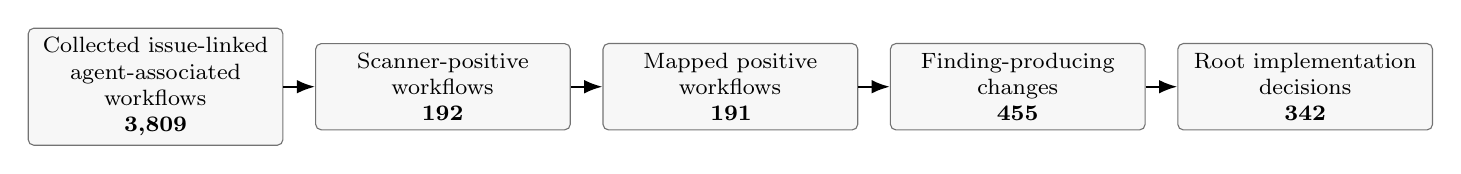
\begin{tikzpicture}[x=1cm,y=1cm,>=Latex,every node/.style={font=\footnotesize}]
\tikzset{stage/.style={draw=black!55,rounded corners=2pt,fill=black!3,align=center,minimum height=1.07cm,text width=3.00cm}}
\node[stage] (a) at (0,0) {Collected issue-linked\\agent-associated workflows\\\textbf{3,809}};
\node[stage] (b) at (3.65,0) {Scanner-positive\\workflows\\\textbf{192}};
\node[stage] (c) at (7.30,0) {Mapped positive\\workflows\\\textbf{191}};
\node[stage] (d) at (10.95,0) {Finding-producing\\changes\\\textbf{455}};
\node[stage] (e) at (14.60,0) {Root implementation\\decisions\\\textbf{342}};
\draw[->,thick] (a)--(b);\draw[->,thick] (b)--(c);\draw[->,thick] (c)--(d);\draw[->,thick] (d)--(e);
\end{tikzpicture}
\caption{Recorded construction and attribution stages. Units change at each stage: workflows are not the same as scanner findings, producing changes, or root decisions. Counts are preliminary historical pipeline results; the latter three are represented by current frozen export files.}
\label{fig:pipeline}
\end{figure*}

\subsection{From scanner finding to producing change}
We distinguish four objects. A \emph{canonical finding} is a scanner-reported condition after study-level deduplication. A \emph{finding-producing change} (PC) is a changed operation, dependency resolution, or artifact to which one or more findings are mapped. A \emph{root decision} groups PCs sharing an underlying implementation choice. A \emph{case} is a workflow; one case may contain many canonical findings, PCs and roots. This separation avoids treating a repeated warning in several files as several independent design decisions.

The intended baseline comparison conceptually tests a finding identity at PR head against a comparable baseline state. For a scanner $S$, an apparent change in alerts may be written as
\begin{equation}
 \Delta_S = \operatorname{Findings}_S(\text{head}) \setminus \operatorname{Findings}_S(\text{base}),
 \label{eq:delta}
\end{equation}
subject to the same enabled analysis, compatible rule versions and defensible matching of warning identities. Equation~\eqref{eq:delta} is a measurement target rather than a guarantee: the current exported cases do not yet supply a complete independently verified baseline/head SARIF trail for every claimed finding. Attribution also requires a path from the changed code to the reported rule, not merely proximity in a diff. The frozen PC packet records location, rule, rationale and relevant source context when available, and missing evidence is treated as an uncertainty rather than silently filled in.

\subsection{Direct effects and supporting side effects}
PCs were coded as \emph{Direct} when the scanner-associated operation implemented the main requested capability, \emph{Side-effect} when it arose in supporting code, tests, dependency updates or auxiliary artifacts, and \emph{Unclear} when evidence did not distinguish the two. These categories describe the relationship to the issue goal, not the security severity of the operation. A scanner report against a test helper can be a side effect and still fail to demonstrate production exposure; a direct change can be innocuous despite matching a scanner rule. Both are possible within the corpus.

\subsection{Root decisions and pre-implementation explanation}
The root census separates \emph{Human-fixed (H)}, where the exact mechanism appears in an eligible pre-implementation human instruction; \emph{Mechanical/toolchain (T)}, where the output follows dependency resolution or generation mechanics without an independently selected mechanism; and \emph{Mechanism-choice (M)}, where alternatives were feasible and the implementer selected a concrete technique. Unresolved roots are tracked separately. The distinctions are operational: \emph{human-fixed} does not prove a human wrote the patch, and \emph{mechanism-choice} does not prove a model selected it.

For M roots, historical analysis used an evidential tier: T1 direct or near-copy reuse; T2 strong repository architecture or precedent; T3 explicit pre-change contract or guidance; T4 contextual plausibility without evidence selecting the exact mechanism; and T5 no independent pre-change explanation after a sufficiently complete search. \emph{Incomplete} is a separate status where the search was not exhaustive. T5 is therefore intentionally difficult to assign. Existing implementation evidence is not automatically evidence the issue reporter supplied it to the implementer: chronology and source accessibility must be checked.

\subsection{Matched workflow controls}
To investigate issue specificity, the pipeline matched scanner-positive workflows to scanner-negative workflows drawn from a comparable scan opportunity. The frozen matched-pair table contains 190 pairs, including 115 same-repository pairs. Its recorded matching features include scanner opportunity, PR timing, changed-line magnitude and changed-file magnitude, with repository identity preferred where possible. These factors reduce some obvious opportunity differences but cannot eliminate differences in task complexity, code paths, exposure, agent tool, code review or unobserved developer context.

Issue specificity is coded from the issue itself: \emph{problem only}, \emph{suggested solution}, or \emph{explicit instruction}. PR alignment is coded separately from the patch: \emph{aligned}, \emph{expanded}, \emph{diverged}, or not assessable. Alignment does not imply security; a perfectly aligned PR can contain a concerning method. Coding must also verify what the issue said at implementation time: later edits to the currently visible issue body and reverse issue/PR chronology can invalidate a claimed pre-implementation instruction.

\subsection{Exploratory intervention design}
Two intervention families were undertaken at different points in the project. First, small precedent experiments selectively exposed or withheld repository context thought to support a specific implementation mechanism. These experiments test sensitivity to the \emph{selected} context, not the absence of all possible information pointing to that mechanism. If equivalent guidance remains in a file or issue, a nominal negative-context condition is not a clean counterfactual.

Second, a retrospective warning-informed replay compared three issue-input conditions: \textbf{O}, the original issue; \textbf{W}, the original issue supplemented with information drawn from a historically observed scanner warning; and \textbf{P}, a more general safety-principle version derived from the same hindsight. P intentionally removes some warning-specific language, but it remains case-specific hindsight guidance rather than an independently available prospective rule. Each replay returns a generated patch whose scanner record is compared with the corresponding control output. The intervention is intended to ask whether missing safety constraints might have made a particular historical failure avoidable. It is \emph{not} a system for knowing a future failure before implementation.

Scanner outcomes and functional outcomes must be evaluated separately. In principle, accepted replays should satisfy the original task requirements, build, pass task-relevant tests and preserve intended behavior. Those complete acceptance judgments are not established for the current archive. Reduced code changes, omitted features or syntax failures are competing explanations for apparently improved scanner outcomes.

\subsection{Evidence handling and review status}
The original 122-case workbook has been independently recounted for descriptive statistics. The current uploaded export was also directly counted for its 455 PC rows, 342 root packets and 190 control pairs. In contrast, scanner-rule correctness, full root adjudication, historical issue text and all paired statistical tests have not been independently reproduced end-to-end in this draft. An earlier workbook named \emph{consensus} consolidated AI-assisted preliminary coding; it cannot be reported as independently completed human review. A separate blind human-review procedure, including full patch and scanner-source inspection, remains scheduled for the post-feedback phase. The Results section therefore distinguishes an exported row count, a historically reported analysis and a verified security conclusion.

\section{Preliminary Results}
\subsection{RQ1: A scanner finding is not an implementation decision}
The first analytical result is a change of unit. The current export has 455 PC records associated with 191 distinct mapped cases; the historical classification reports 134 Direct, 318 Side-effect and three Unclear PCs. These sum to 455. In the previously reviewed 122-case subset, the primary workbook recount finds 605 canonical findings collapsed into 322 PCs, of which 91 were Direct, 228 Side-effect and three Unclear. The reported 70-case extension contributes a further 133 PCs, giving the full 455-PC total. This arithmetic reconciliation supports internal consistency without confirming that each scanner report describes an independently exploitable weakness.

The project further groups PCs into a reported 342 root decisions. Table~\ref{tab:root} contains the current historical classification. Mechanism-choice roots are the largest group, but the table cannot establish who exercised the choice or whether the choice caused a genuine security weakness. The M-tier breakdown is especially sensitive to evidence completeness. An earlier selected 55-root coding is not interchangeable with the eventual 342-root census; an additional audit revised eleven previous T5 assignments to nine T4 and two incomplete, illustrating how absence-of-evidence conclusions change with source coverage.

\begin{table}[t]
\centering\footnotesize
\caption{Reported implementation-root classification (342 roots). Counts are historically recorded, not yet independently re-adjudicated.}
\label{tab:root}
\begin{tabularx}{\columnwidth}{@{}Xr@{}}\toprule
\textbf{Route} & \textbf{Roots}\\\midrule
Human-fixed mechanism (H) & 6\\
Mechanical/toolchain effect (T) & 103\\
Discretionary mechanism choice (M) & 233\\\midrule
\textbf{Total} & \textbf{342}\\\midrule
\multicolumn{2}{@{}l}{\emph{Within the 233 M roots (reported):}}\\
T1 near-copy or direct reuse & 32\\
T2 strong repository precedent & 12\\
T3 binding pre-change contract & 33\\
T4 contextually plausible only & 128\\
T5 no independent precursor found & 4\\
Incomplete evidence search & 24\\\bottomrule
\end{tabularx}
\end{table}

The original issue-risk sheet assigned 117 of 122 cases to benign ordinary and five to benign ambiguous, with none assigned a malicious category. These are \emph{provisional study labels}: the workbook's independent human correction fields were blank. They do not establish either malicious prevalence or the absence of malicious attacks outside a scanner-positive gate.

\subsection{Illustrative cross-artifact cases}
An example illustrates why our objects must be kept distinct. In \ncase{3375} (\url{https://github.com/caliber-ai-org/ai-setup/pull/17}), an issue concerns a Node.js deprecation warning affecting command execution on Windows. The archived PR changes the shell invocation strategy, and a Semgrep rule reports use of \texttt{child\_process} in a changed editor utility. The observable chain is therefore an issue requirement, a concrete changed implementation, and a scanner signal. It is \emph{not}, without reachability and input-control evidence, a verified command-injection exploit. The case also illustrates that the issue's relation to secure shell use can be explicit while the exact patch technique is still a choice to investigate.

Another archived case, \ncase{12313} (\url{https://github.com/weapp-vite/weapp-vite/pull/729}), concerns Vue component compilation. Its mapped scanner record describes a regular-expression warning in an end-to-end test file, including failure to match uppercase \texttt{SCRIPT} tags. This is useful evidence about the scanner's operational selection rule, but a test-only regex should not be silently treated as evidence that production users can exploit an HTML-filtering weakness. These examples motivate human assessment of artifact role and attacker reachability before security conclusions.

\subsection{RQ2: Issue specificity and matched controls}
The historically recorded 190-pair analysis reports that explicit implementation instructions appeared in 63.7\% of scanner-positive issues and 77.9\% of matched scanner-negative controls. In the 115-pair same-repository sensitivity set, the reported percentages were 67.0\% and 82.6\%, respectively. This direction is compatible with a specification-gap hypothesis: more constrained tasks may leave less room for an implementation mechanism to be selected without guidance. However, it is also compatible with differences in task composition, codebase characteristics, selection by scanner rules, or imperfect matching. The percentages and $p$ values in Table~\ref{tab:matched} are outputs from the historical comparison and have not been independently recalculated for this draft.

\begin{table}[t]
\centering\footnotesize
\caption{Historical scanner-positive vs. matched-control comparisons. These are reported descriptive analyses, not causal effects or final certified tests.}
\label{tab:matched}
\begin{tabularx}{\columnwidth}{@{}Xrr@{}}\toprule
\textbf{Measure} & \textbf{Positive} & \textbf{Control}\\\midrule
Explicit issue instruction, all pairs & 63.7\% & 77.9\%\\
Explicit issue instruction, same repo & 67.0\% & 82.6\%\\
PR aligned with issue, all pairs & 84.2\% & 96.3\%\\\bottomrule
\end{tabularx}
\vspace{2pt}\parbox{\columnwidth}{\scriptsize Reported paired tests: specificity $p=0.00052$ overall, $p=0.00645$ same repo; alignment $p=0.001$ overall but $p=0.077$ in the same-repository subset. The test inputs and coding require re-audit.}
\end{table}

Reported PR alignment is also lower for positives in the full matched sample (84.2\% versus 96.3\%). However, its same-repository test was not conventionally significant ($p=0.077$). We therefore treat PR alignment as a sensitivity-limited descriptive contrast, not a second confirmed explanatory result. Several broader metadata comparisons, including issue purpose, review patterns, delay, contributor activity and agent-tool type, did not show comparably clear evidence of differences in the historical tests. Failure to detect a difference is not proof of equivalence.

A decision-level comparison separately reported visible checks or guards in 29 of 31 selected positive roots versus ten matched controls. But roughly 21 of 31 positives had a guard/check construct that overlapped with the operational scanner rule. This is an important alternative explanation: a scanner may select exactly the construct that a separate coder labels as a check. Thus the contrast may be partially definitional and is not used as independent evidence that validation checks create vulnerabilities.

\subsection{RQ3: Retrospective safety guidance and context}
Table~\ref{tab:owp} summarises the archived retrospective warning-guidance comparison. The archive contains 14 cases and 40 recorded arm-level scans: 12 O runs, 14 W runs and 14 P runs. Only 12 cases have a complete three-arm comparison. In that paired subset, the recorded counts of outputs with zero \emph{claimed newly introduced} CodeQL alerts are 2/12 for O, 5/12 for W and 5/12 for P. The corresponding reported sums of new alerts are 21, ten and 15. These are records of the archival scoring process, not independently reconstructed base/head scanner deltas.

\begin{table}[t]
\centering\footnotesize
\caption{Exploratory retrospective issue-guidance replay: 12 complete O/W/P cases. A zero-alert patch is not necessarily functional or secure.}
\label{tab:owp}
\begin{tabularx}{\columnwidth}{@{}Xrr@{}}\toprule
\textbf{Input arm} & \textbf{Zero recorded new alerts} & \textbf{Recorded new alerts}\\\midrule
O: original issue & 2/12 & 21\\
W: original + historical warning & 5/12 & 10\\
P: original + generalised principle & 5/12 & 15\\\bottomrule
\end{tabularx}
\end{table}

The interpretation is deliberately limited. The archive lacks a complete set of before-scan SARIF artifacts needed to independently reproduce every new-warning delta. The replays also do not establish equal coverage of the original task. W and P generally have smaller patches than O, and one original-condition output passed the zero-new-alert criterion despite failing a recorded syntax check. Even if the warning-inspired condition suppressed a scanner rule, it might have omitted work instead of producing a correct safer implementation. Moreover, W is a hindsight oracle: a new issue's author would not normally know the exact warning a not-yet-generated patch will trigger. P removes some warning syntax but was still chosen with knowledge of the historical case. These data motivate, but do not prove, prospective safety-specification benefits.

Context-precedent experiments were likewise mixed. An early six-root pilot recorded the targeted mechanism in 4/15 no-X versus 9/15 with-X outputs (exploratory $p\approx0.068$). A later strict, four-pair bidirectional comparison recorded no corresponding within-side change: positives 4/8 versus 4/8, negatives 0/8 versus 0/8. Because omitting a selected precedent did not reliably remove equivalent mechanism information from other parts of the task, this is not a clean experiment on \emph{all} relevant context. Together the studies support an uncertainty-aware research direction, not a mechanism-level causal conclusion.

\section{Discussion}
\subsection{What the evidence presently supports}
The descriptive mapping shows why issue-centered analysis should not end at a scanner alert. A workflow can yield multiple alerts from one implementation choice, or several distinct supporting operations whose relation to the requested goal differs. The reported predominance of M roots suggests that mechanism selection is an important object of study. Nevertheless, attribution of a decision to an LLM rather than a human collaborator is not established merely because the repository or PR bears an agent marker. The defensible statement is about \emph{agent-associated workflows and observable changes}.

The matched-control comparisons provide preliminary support for investigating specification detail, especially because the direction of the instruction-specificity contrast persists in the reported same-repository subset. They do not demonstrate that adding instructions would prevent warnings. The scanner-positive sampling rule, task type and availability of comparable negatives may shape the difference. The guard/check example is a warning against post-hoc explanatory storytelling: a strong association can arise because the outcome-selection instrument and purported explanation detect the same implementation structure.

The retrospective warning interventions are best viewed as \emph{diagnostic counterfactual probes}. They ask whether a known scanner-associated failure might be avoidable under more informative task context. That question is scientifically useful even if the input is an oracle that cannot be deployed prospectively. The eventual practical goal would instead require formulating \emph{ex ante} constraints that a maintainer can reasonably know before seeing the patch, then testing functional fidelity and genuine security outcomes. The current data do not identify a universal minimal instruction set or reliable early-warning policy.

\subsection{How the original malicious-issue question changes}
Our initial motivation concerned intentionally poisoned GitHub issues. The historical real-world triage did not uncover affirmative maliciousness within its sampled positive set. That observation is restricted by its lack of completed independent human review and by the scanner gate, which may exclude evasive attacks that produce no new detectable alert. Absence of malicious labels in this subset cannot estimate attack prevalence in the larger issue population. Controlled attack datasets remain valuable as positive cases for testing annotation definitions, but their constructed nature cannot substitute for authentic real-world ground truth.

This distinction also sharpens the study's contribution. We are not claiming to have discovered a previously unknown population of attackers. We are describing a way to study \emph{agent-steering opportunity and implementation discretion} without collapsing them into malicious intent. A benign issue can create an unconstrained decision point. Whether an adversary exploits that point is a different, evidence-hungry claim.

\subsection{Implications for empirical measurement}
Three concrete refinements follow. First, the dataset should retain the exact issue version visible before implementation; issue-body edits and the order of timestamps affect whether a specification could have influenced the patch. Second, a finding record should include the scanner version, matched base/head evidence, affected changed hunk, and human security assessment; a scanner label alone is insufficient. Third, interventions must measure task success jointly with scanner outcomes, with comparable patch scope, complete generation provenance and clean controls. These are proposed measurement improvements, not new completed results.

The current corpus also suggests that explanation tiers should be confidence- and completeness-aware. A T4 decision is not \emph{causally explained} simply because surrounding code makes it understandable; a T5 code requires evidence that eligible precursors were searched and absent. The later historical reclassification of old T5 cases demonstrates how much methodological care the distinction requires. This kind of negative-result and correction tracking is part of the reproducibility contribution, not an inconvenience to omit.

\section{Threats to Validity}
\textbf{Construct validity.} Scanner detections mix code flows, dependency advisories, suspicious strings and test artifacts. Their meaning depends on rule semantics, attacker control and runtime reachability. A matched scanner-negative workflow is not known vulnerability-free. "Agent-associated" derives from observable GitHub markers and is not proof of autonomous patch authorship. "Human-fixed", "mechanical" and "mechanism-choice" are evidence classifications, not process-trace observations.

\textbf{Internal validity.} The matched study remains observational. Matching on scanner opportunity, repository, time and changed diff magnitude does not balance latent complexity, developer expertise or code coverage. The scanner rule can overlap a coded guard/check predictor. Current issue text can differ from the issue as it existed when the PR was prepared; four historical 122-case PR timestamps predate the linked issue timestamps, requiring explicit chronology checks before causal ordering claims. Retrospective interventions use hindsight and may contain persistent equivalent mechanism cues, invalidating simple treatment contrasts.

\textbf{Conclusion validity.} The 190-pair statistics have not yet been freshly recomputed from raw labels in this manuscript version. Small experiments have limited power; exploratory $p$ values should not be treated as confirmatory. Repeated generations from the same case are not interchangeable with independent cases. In the O/W/P study, original versus modified outputs varied in patch size and potentially in completed functionality. Counts of zero scanner alerts cannot estimate secure, successful repair.

\textbf{External validity.} Inclusion relied on merged, issue-linked public PR workflows, observable agent-use markers, repository selection criteria and specific scanners. Unmerged proposals, invisible agent activity, private repositories, and scanner-evasive malicious issues may be systematically absent. The studied sampling window does not support ecosystem-wide prevalence estimates. Moreover, a control from another repository may have substantially different security-relevant architecture.

\textbf{Measurement and review reliability.} Root/PC joins are represented by exported evidence, but the final D-level labels, scanner introduction status, warning rule equivalence and historical issue chronology are not uniformly reverified. The 122-case issue-risk workbook had no completed independent human correction fields. AI-assisted preliminary consensus must not be called blinded independent human adjudication. A publication version requires a frozen codebook, independently coded subset, disagreement adjudication, audit trails and exact reproducibility manifests.

\section{Conclusion and Future Work}
This exploratory study investigates a narrower and more defensible question than the presence of malicious issue authors: how issue text, repository context and implementation choice relate to scanner-reported conditions in agent-associated public PR workflows. The present evidence includes a recorded collection of 3,809 issue-linked workflows, an exported 455-change attribution set, and a 190-pair matched-control design. Historical analyses suggest that scanner-associated changes often involve supporting artifacts and discretionary mechanisms, and that issues associated with scanner-positive workflows may provide less explicit implementation guidance. These are descriptive and observational findings, not estimates of exploitability, attacker prevalence or causal prevention.

A further retrospective replay suggests that adding warning-derived guidance can alter recorded scanner outcomes in selected cases, but incomplete scanner baselines, functional acceptance and patch-size equivalence prevent a security-improvement claim. The immediate next research phase is therefore not indiscriminate expansion. It is evidence consolidation: independently reproduce the cluster statistics; link base/head scanner artifacts to exact changed code; complete blind human review; and construct a versioned, properly labelled dataset incorporating original issues, code context, agent traces when available, and carefully separated controlled-attack examples. Those steps can strengthen or revise the present findings without requiring the first supervisor-feedback draft to pretend that all uncertainties are resolved.

\balance
\bibliography{references}
\end{document}
